

\begin{frame}

\end{frame}


\begin{frame}{Non-maximum Suppression}
    \begin{figure}
        \centering
        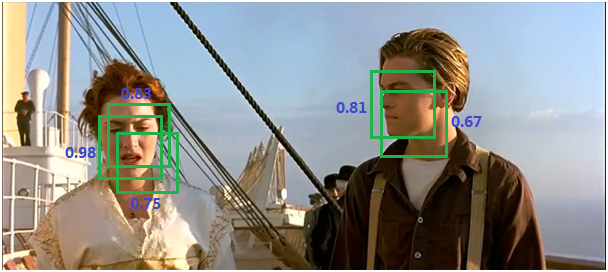
\includegraphics[scale=0.4]{nms1.png}
        \caption{Before NMS}
    \end{figure}
    
    \begin{figure}
        \centering
        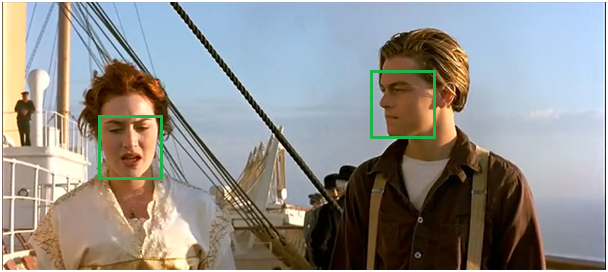
\includegraphics[scale=0.3]{nms2.png}
        \caption{After NMS}
    \end{figure}
\end{frame}

\begin{frame}{Bounding-box Regression}
    Green box: the ground truth bounding box; \\
    Red box: selective search region proposal; \\
    
    \begin{figure}
    \centering
    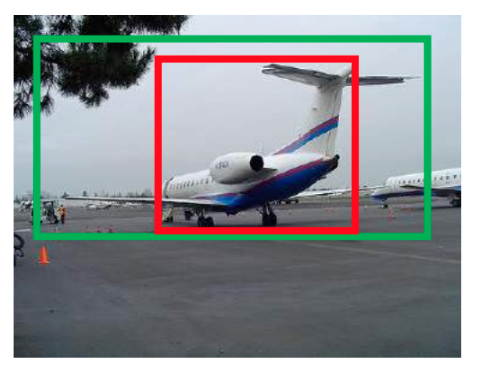
\includegraphics[scale=0.3]{img1.png}
    \end{figure}
    
    Bounding-box regression is used to adjust the red box to make it as close 
    as possible to the green one.
\end{frame}


\begin{frame}{YOLO v3 Model}
    \begin{itemize}
        \item Backbone network: Darknet-53;
        \item Anchor: total 9, but 3 for each scale;
        \item Logistic vs. Softmax: support multi-label classification;
        \item Objectness score for each box instead of each location;
    \end{itemize}
    \begin{figure}
        \centering
        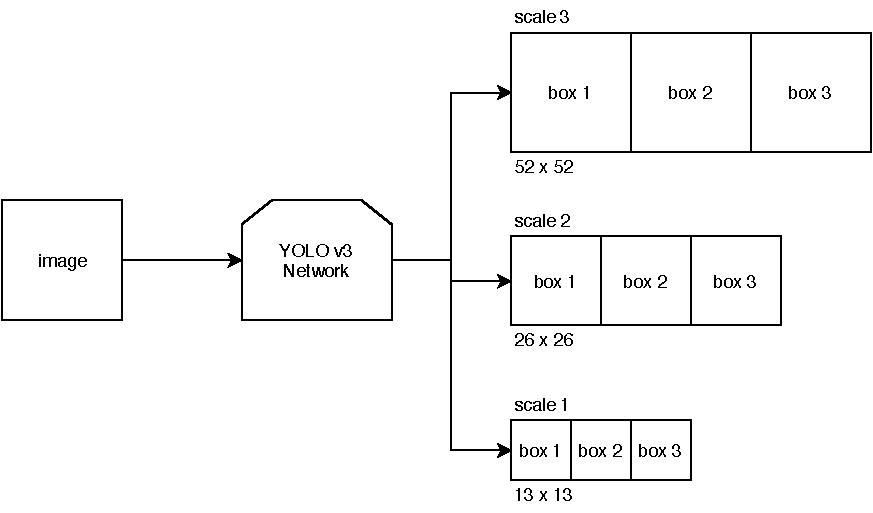
\includegraphics[scale=0.5]{yolov3_network.pdf}
        \caption{YOLO v3 process flow.}
    \end{figure}
\end{frame}

\begin{frame}{Detector Instantiation}
    \begin{figure}
        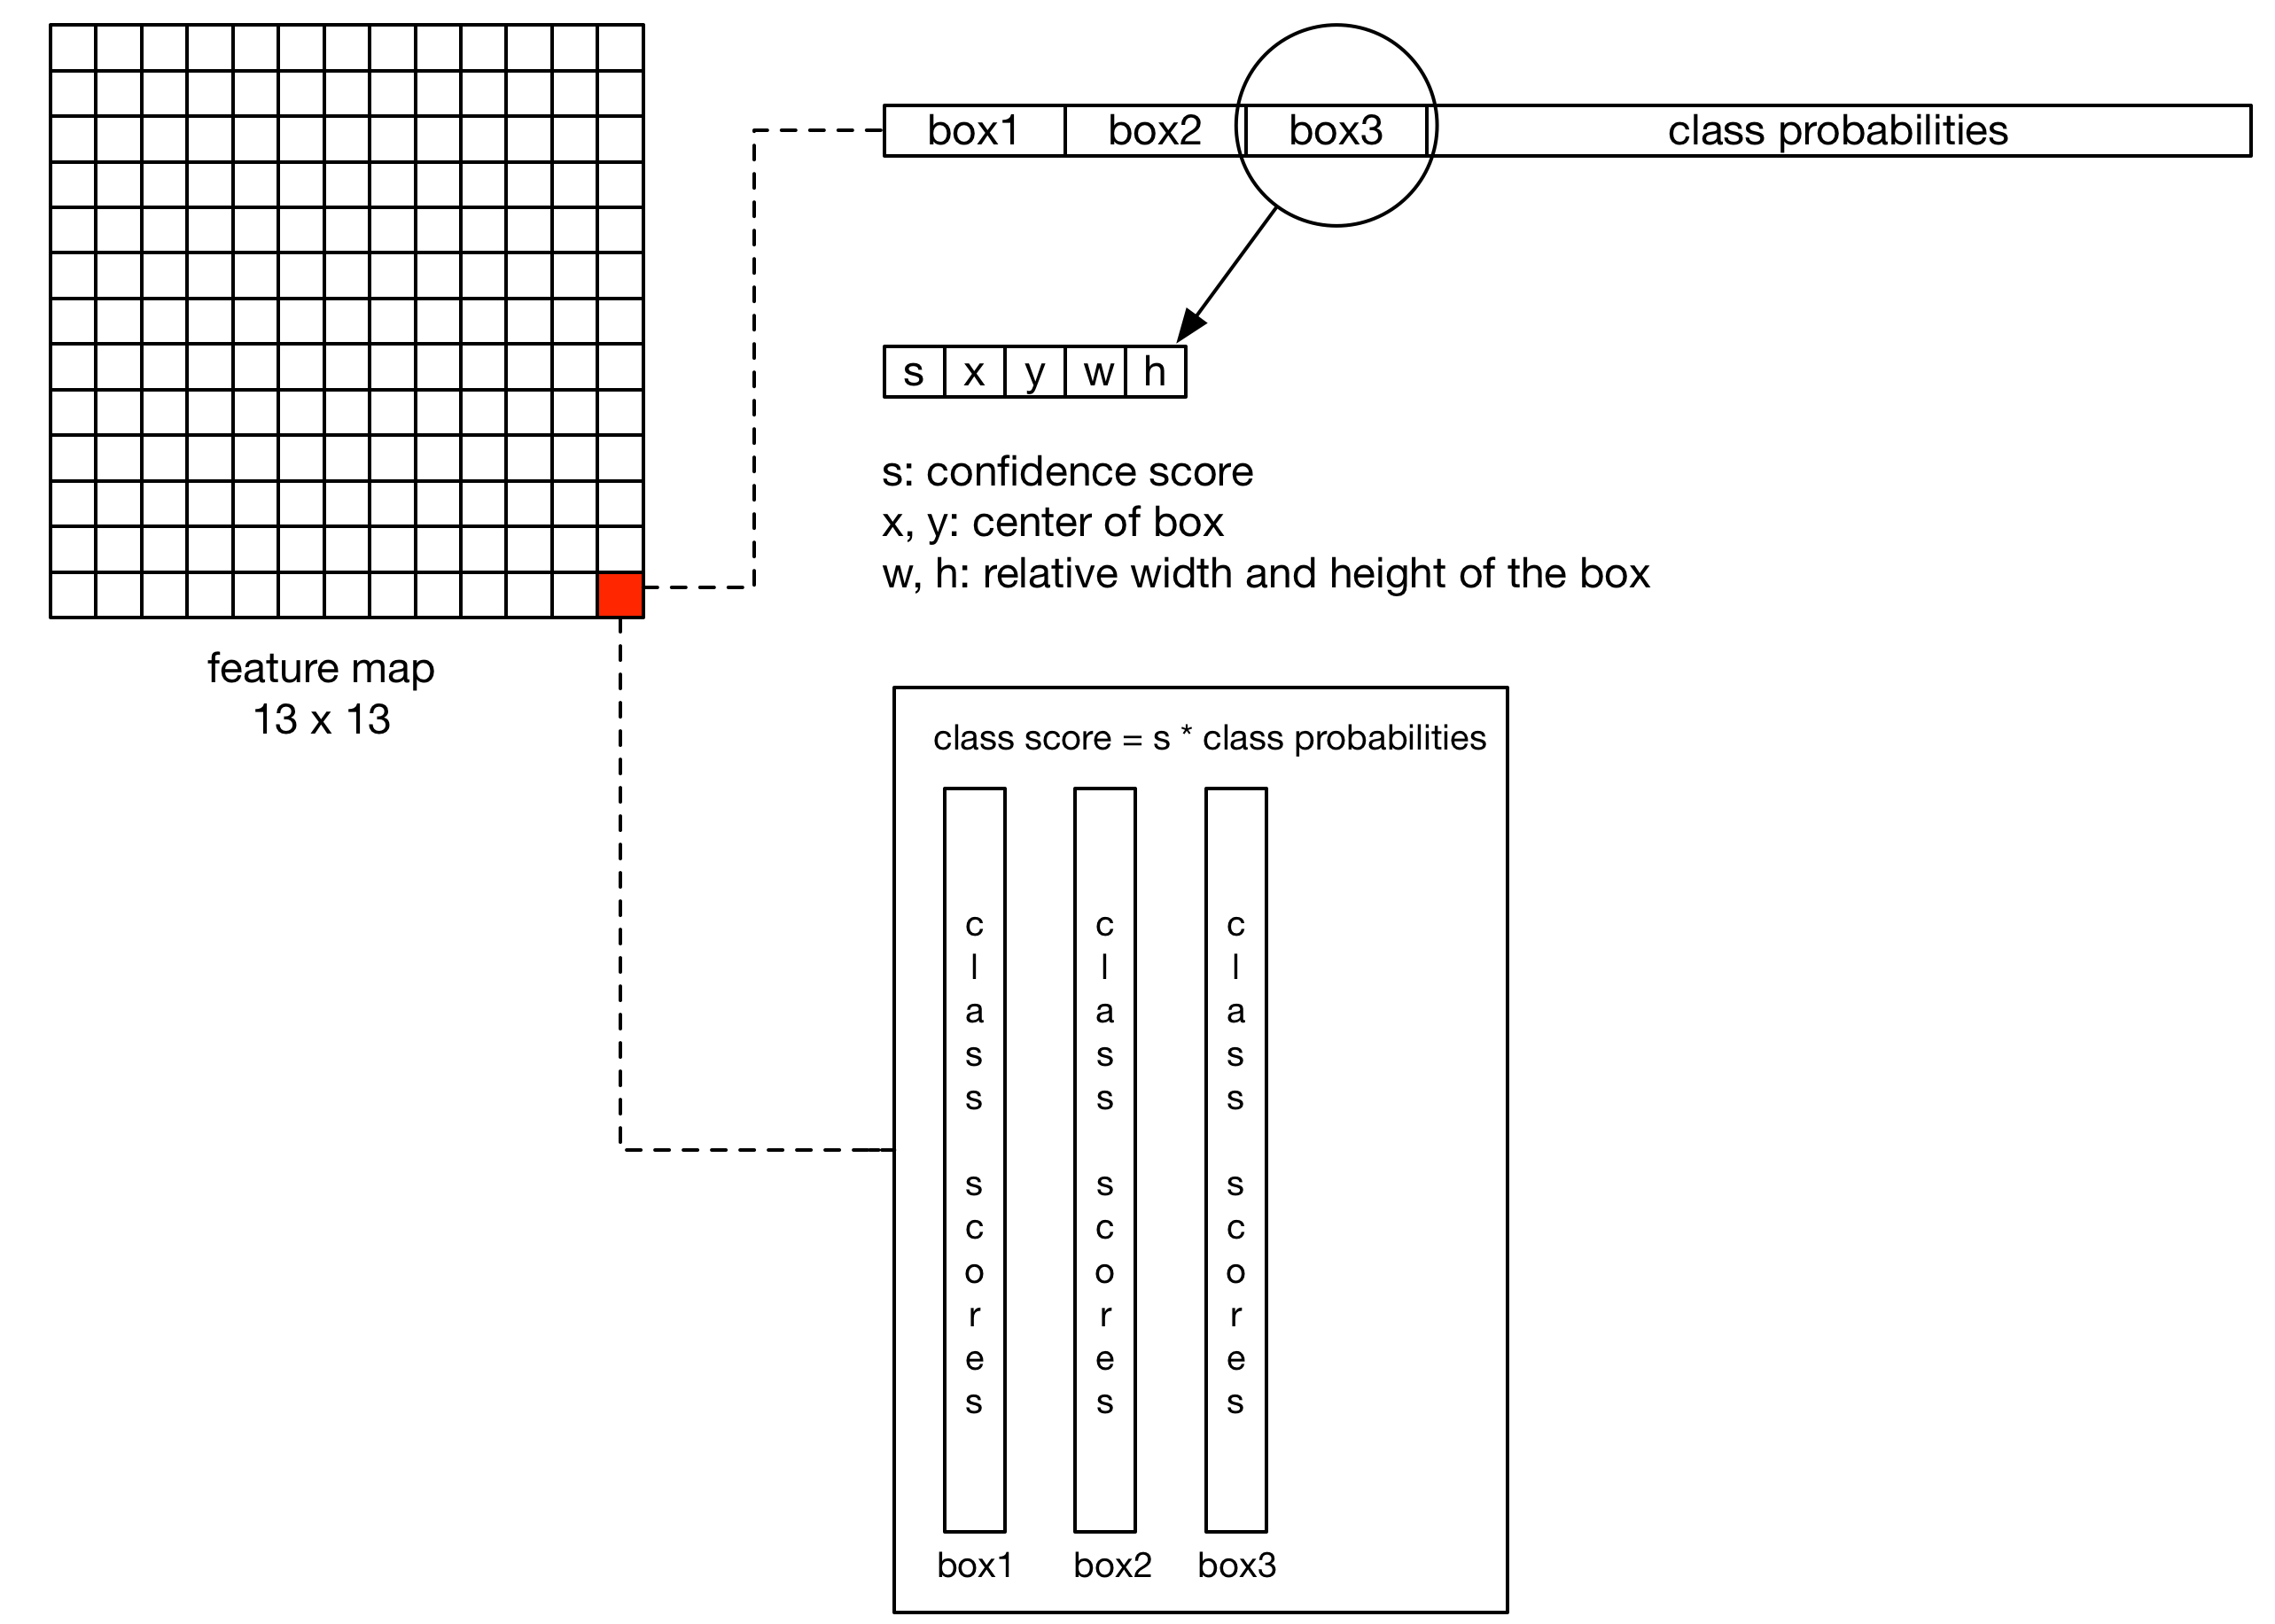
\includegraphics[width=\linewidth]{framework_detector_calc.png}
        \caption{Calculation process of each cell in the feature map.}
        \label{fig:fw-detector-calc}
    \end{figure}
\end{frame}

\begin{frame}{Detector Instantiation}
    \begin{figure}
        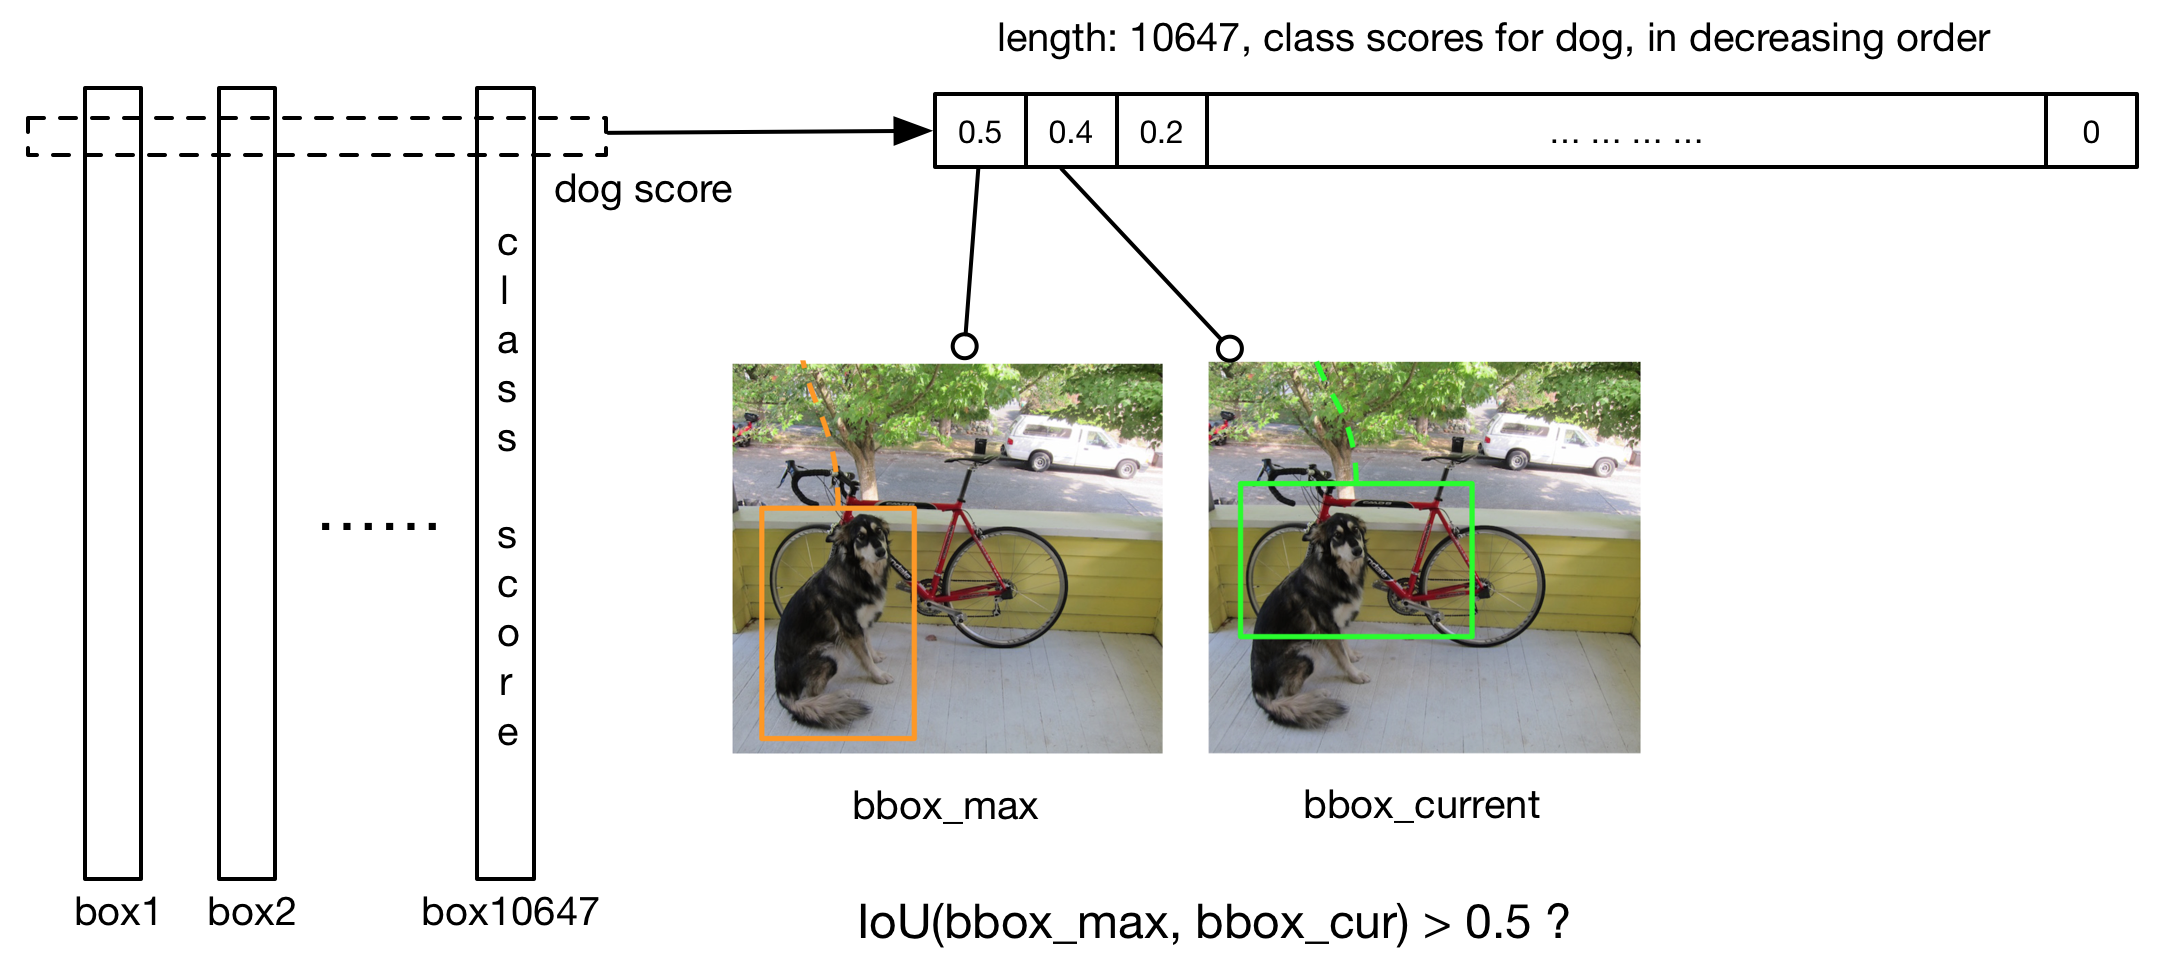
\includegraphics[width=\linewidth]{framework_detector_nms.png}
        \caption{Non-maximum suppression process.}
        \label{fig:fw-detector-nms}
    \end{figure}
\end{frame}

\begin{frame}{Person Detector Evaluation}
    \textbf{Intersection over Union Overlap}\\
    \vspace{10px}
    Intersection over Union Overlap (IoU) is used to measure how close a given 
    bounding box is to another box that is independent of the units used 
    (pixels, etc).
    \vspace{10px}
    \begin{figure}
        \centering
        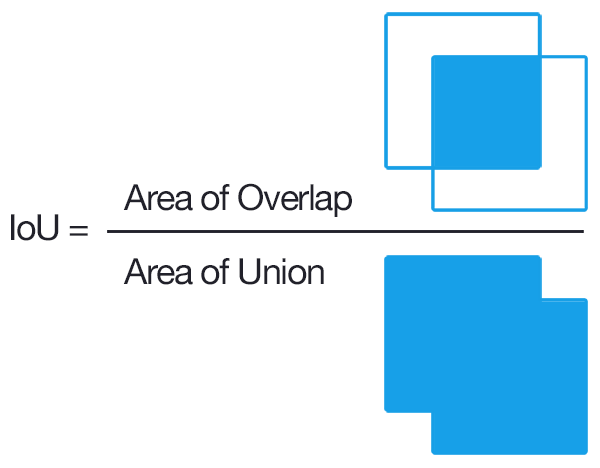
\includegraphics[scale=0.2]{iou.png} 
    \end{figure}
\end{frame}

\begin{frame}{Person Detector Evaluation}
    Possible results for one detection operation:
    \begin{itemize}
        \item True positive, a correct detection where $\mathit{IOU} \geq
        \mathit{threshold}$.
        \item False positive, a incorrect detection where $\mathit{IOU} <
        \mathit{threshold}$.
        \item True negative, does not apply.
        \item False negative, a ground truth not detected.
    \end{itemize}
\end{frame}

\begin{frame}{Person Detector Evaluation}
\textbf{Precision and Recall}\\
\vspace{5px}
\begin{description}
    \item[Precision] 
    is a fraction of relevant instances among the retrieved instances which can 
    be used to measures how accurate is your prediction.
    \item[Recall]
    is a fraction of relevant instances that have been retrieved over the total 
    amount of relevant instances. It can be used to measure how good you find 
    all the positives.
\end{description}

$$
\mathit{precision} =
\frac
{\text{\# true positive}}
{\text{\# true positive + \# false positive}}
$$

$$
\label{eq:recall}
\mathit{recall} =
\frac
{\text{\# true positive}}
{\text{\# true positive + \# false negative}}
$$
\end{frame}

\begin{frame}{Person Detector Evaluation}
    With precision and recall in hand, we can construct a Precision-Recall curve
    (P-R curve) which will be used to calculate our metric. The curve
    construction process can be described as the following:
    
    \begin{enumerate}
        \item Collect all the predictions that make for a particular class of
        objects. Rank them in decreasing order according to the confidence score
        given by the model.
        \item  Compare theses predictions with ground truth to see if they are 
        correct or not.
        \item Calculate the precision and recall using the given formula for 
        each prediction in the ranked list from top to bottom.
    \end{enumerate}
\end{frame}

\begin{frame}{Person Detector Evaluation}
    \begin{figure}
        \centering
        \begin{minipage}[b]{0.65\textwidth}
            \centering
            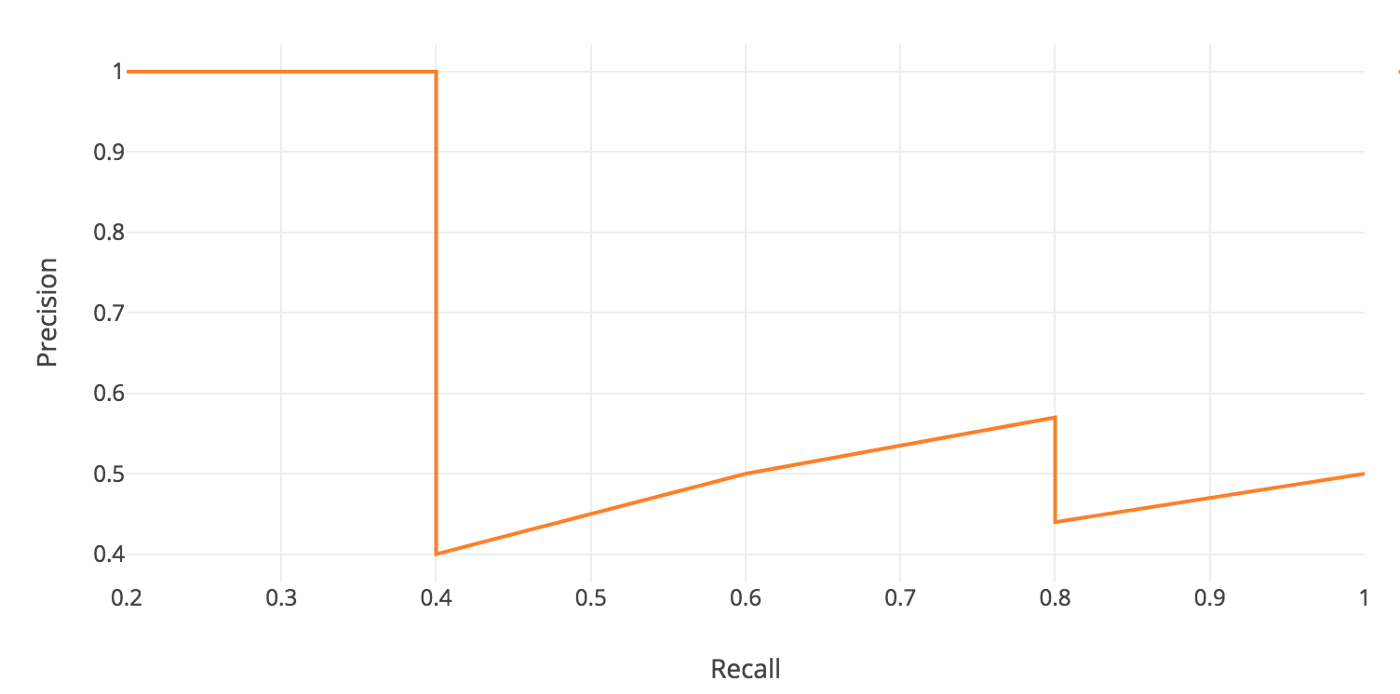
\includegraphics[width=\linewidth]{eval_pr_curve.png}
        \end{minipage}%
        \begin{minipage}[b]{0.35\textwidth}
            \centering
            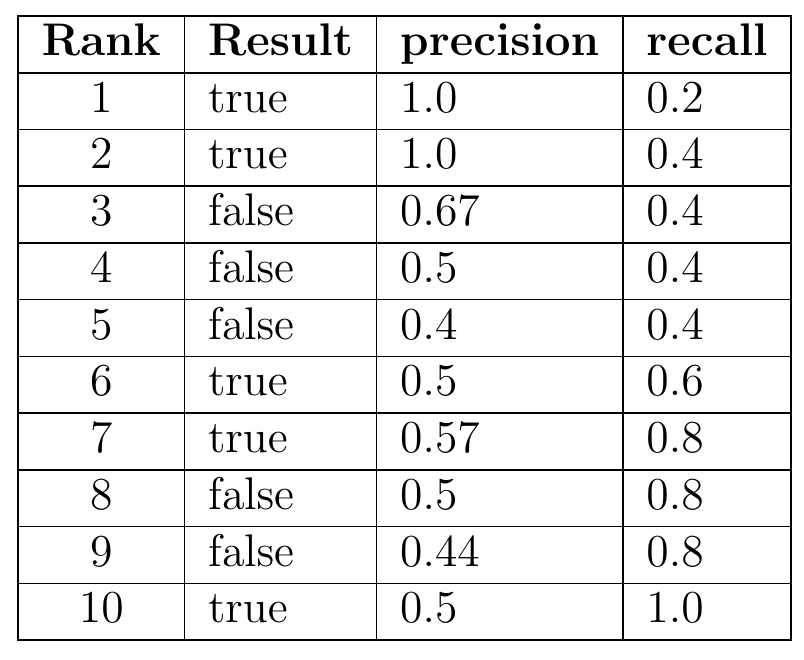
\includegraphics[width=\linewidth]{eval_pr_curve_data.png}
        \end{minipage}
        \caption[An example of Precision-Recall curve]
        {An example of P-R curve. Left is the curve itself and right is the data
            used to plot this curve, assuming that there is a total of five 
            positives
            in the data.}
        \label{fig:eval-pr-curve}
    \end{figure}
\end{frame}

\begin{frame}{Person Detector Evaluation}
    \begin{figure}
        \centering
        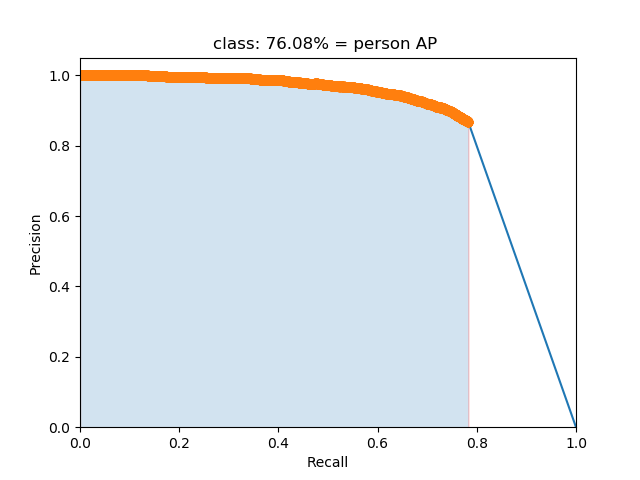
\includegraphics[scale=0.25]{eval_detector_pr_curve.png}
        \caption{Person detection model's Precision-Recall curve on 
            validation set.}
        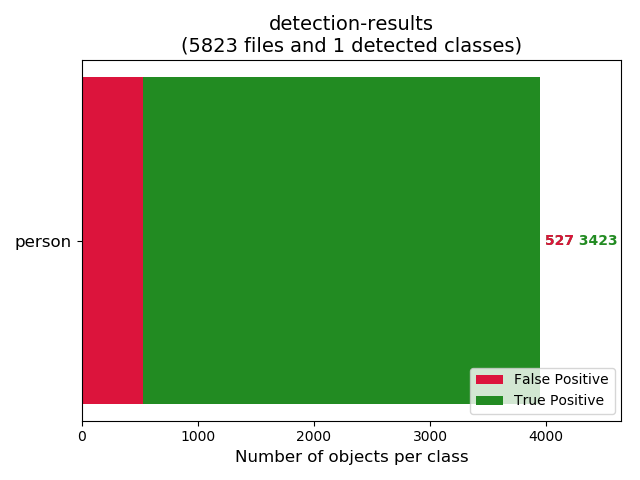
\includegraphics[scale=0.25]{eval_detector_result.png}
        \caption{Person detection result on validation set.}
    \end{figure}
\end{frame}

\begin{frame}{Person Detector Evaluation}
    \begin{figure}
    \centering
    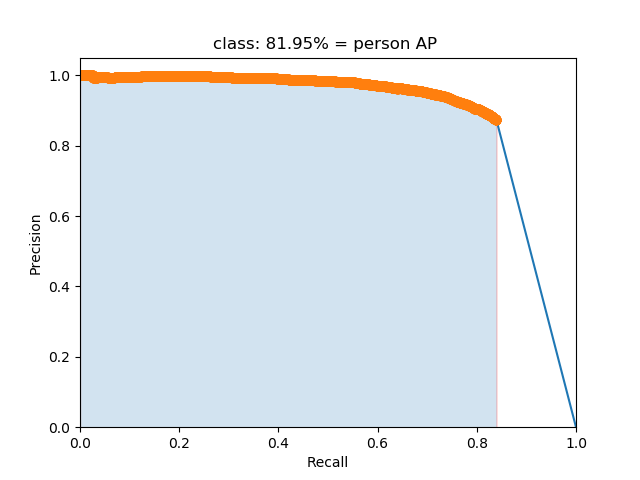
\includegraphics[scale=0.25]{eval_detector_pr_curve1.png}
    \caption{Object detection (with 20 classes supported)\\ 
        model's Precision-Recall curve on validation set.}
    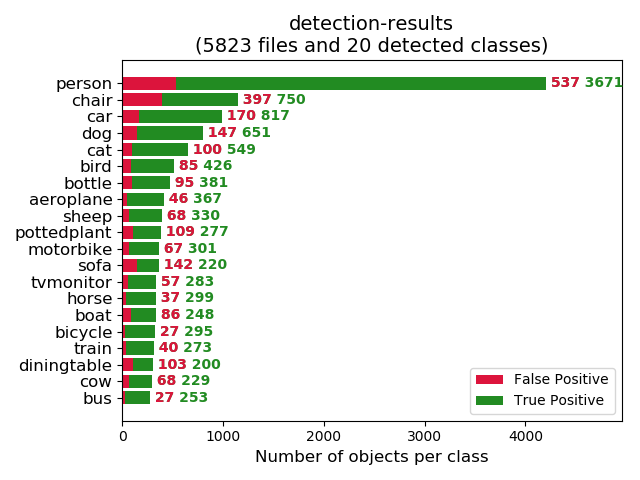
\includegraphics[scale=0.25]{eval_detector_result1.png}
    \caption{Object detection result on validation set.}
    \end{figure}
\end{frame}







\begin{frame}{Recognizer Network Architecture}
    \begin{figure}
        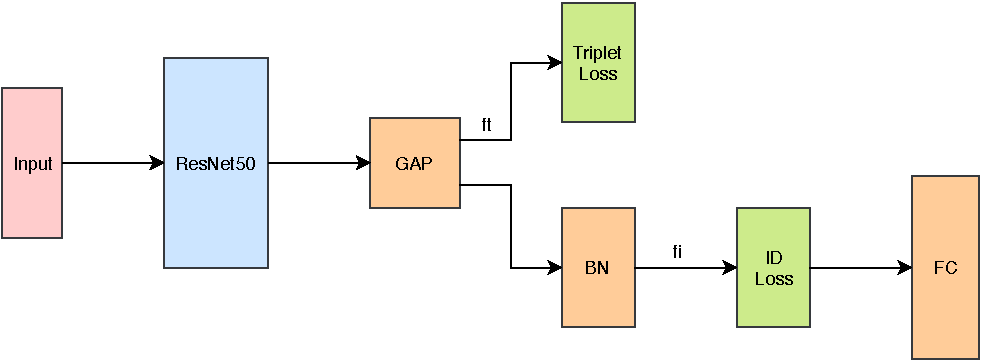
\includegraphics[width=\linewidth]{framework_reid_archit.pdf}
        \caption[Implemented recognizer network architecture]
        {
            Implemented recognizer network architecture.
                    GAP: global average pooling layer, BN: batch normalization
                    layer, FC: fully connected layer.
                    $f_t$: features used to calculate triplet loss,
                    $f_i$: features used for inference.
            The pink color represents input, blue means backbone network, 
            orange represents a special layer and green means loss function 
            layer.
        }
    \end{figure}
    \blfootnote{
        The architecture was proposed in 
        \cite{tricks-and-baseline-for-reid-2019}.}
\end{frame}


\begin{frame}{Recognizer Training Workflow}
    \begin{figure}
        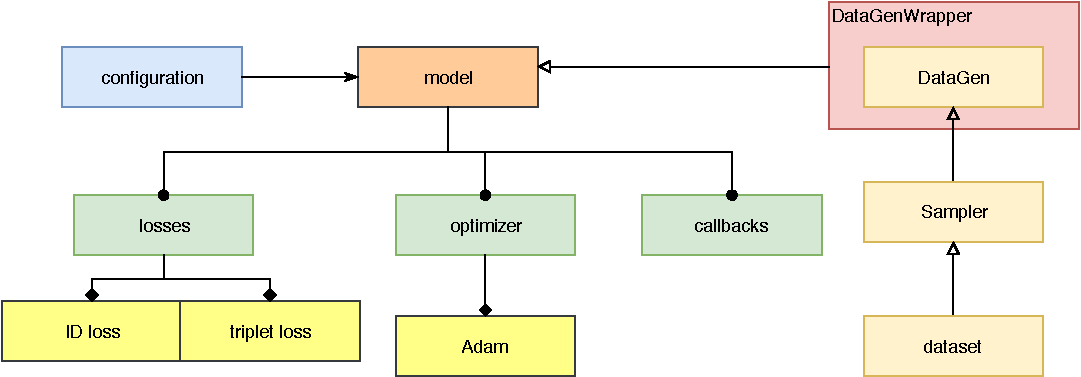
\includegraphics[width=\linewidth]{framework_reid_code_overview.pdf}
        \caption{The workflow of the ReID training program}
    \end{figure}
\end{frame}

\begin{frame}{Recognizer Training}
    \begin{itemize}
        \item batch size: $16 \times 4 = 64$
        \item warm up learning rate strategy \cite{learning-rate-warmup-2018}
        \item triplet loss + ID loss
        \item Adam optimizer
        \item total training epochs 120 \cite{tricks-and-baseline-for-reid-2019}
    \end{itemize}

    $$
        \operatorname{lr}(t)=\left\{
        \begin{array}{ll}
        {3.5 \times 10^{-5} \times \frac{t}{10}} & {\text { if } t \leq 10} \\
        {3.5 \times 10^{-4}} & {\text { if } 10<t \leq 40} \\
        {3.5 \times 10^{-5}} & {\text { if } 40<t \leq 70} \\
        {3.5 \times 10^{-6}} & {\text { if } 70<t \leq 120}
        \end{array}\right.
    $$
    
\end{frame}

\begin{frame}{Recognizer Training Visualization}
    \begin{figure}
    \begin{columns}
        \begin{column}{0.4\textwidth}
            \centering
            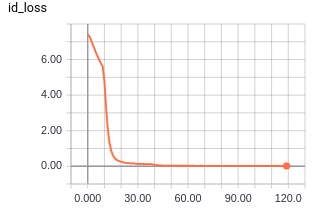
\includegraphics[width=\linewidth]{train_id_loss.png}\\
            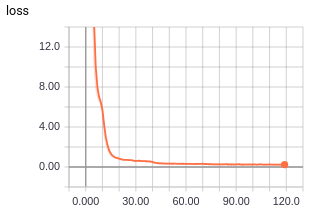
\includegraphics[width=\linewidth]{train_loss.png}
        \end{column}        
        \begin{column}{0.4\textwidth}
            \centering
            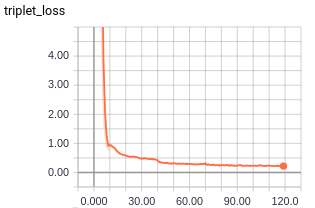
\includegraphics[width=\linewidth]{train_triplet_loss.png}\\
            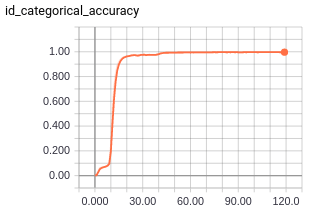
\includegraphics[width=\linewidth]{train_acc.png}
        \end{column}
    \end{columns}
    \caption
    {Training visualization diagram. Upper left: training identification 
        loss curve. Upper right: training triplet hard loss curve. Lower 
        left: total training loss curve. Lower right: training 
        classification accuracy.}
    \end{figure}
    \blfootnote{These figures are produced by the TensorBoard program.}
\end{frame}












































